
%%
%% nb: use pdflatex to create pdf file with hyperlinks
%%

%% =====================================================================
%% DOCUMENT DATA
%% =====================================================================

\documentclass[11pt]{article}

\title{Specifying Grammars for OpenCCG: \\ A Rough Guide}
\author{Cem Boz\c{s}ahin \and Geert-Jan M. Kruijff \and Michael White}


%% =====================================================================
%% PACKAGES
%% =====================================================================

\usepackage{openccg} % for hlds/ccg
\usepackage{graphicx} % for figs
\usepackage{gb4e} % for examples

\usepackage[
  colorlinks=true, linkcolor=blue, citecolor=blue, urlcolor=blue,
  pdfstartview=FitH,
  pdftitle={Specifying Grammars for OpenCCG: A Rough Guide},
  pdfauthor={Cem Bozsahin, Geert-Jan M. Kruijff and Michael White}
]{hyperref}


%% =====================================================================
%% NEW COMMANDS
%% =====================================================================

%\newcommand{\occg}{\textsf{OpenCCG}}
\newcommand{\occg}{OpenCCG}
\newcommand{\tccg}{\textsf{tccg}}

 
%% =====================================================================
%% DOCUMENT BODY
%% =====================================================================

\begin{document}

\thispagestyle{empty}
\maketitle
\tableofcontents
\listoftables
\listoffigures
\newpage

\section{OpenCCG} 

\occg\ is an open source natural language processing library written in
Java, which provides parsing and realization services based on Mark
Steedman's Combinatory Categorial Grammar (CCG) formalism
\cite{Steedman:SynProc}. The library makes use of the multi-modal
extensions to CCG devised by Jason Baldridge in his dissertation
\cite{Baldridge:2002} and in a joint EACL-03 paper with Geert-Jan
Kruijff \cite{Baldridge/Kruijff:2003}. For a concise introduction to CCG
with these extensions, see \cite{Steedman/Baldridge:2003}.

\occg\ grew out of the Grok system developed by Gann Bierner and Jason
Baldridge, and has been refined and extended by Michael White, with
further contributions from Cem Boz\c{s}ahin, G\"une\c{s} Erkan,
Geert-Jan Kruijff, David Reitter and Alexandros Triantafyllidis. Recent
development efforts, managed by Michael White, have focused on making
the realizer
\cite{White/Baldridge:2003,White-RLAC:2004,White-INLG:2004,White-ACLSoft:2005}
practical to use in dialogue systems, and improving (somewhat) the grammar
development process.

You can download and install \occg\ from its website, located at
\url{http://openccg.sourceforge.net}. Once you've unpacked the archive,
have a look at the \texttt{README} file for installation
instructions.


\section{About this (rough) guide}

This guide is intended to provide a brief introduction to writing grammars for
\occg. The system is implemented in Java, but you do not need to know Java.
\occg\ provides its own formats for describing grammars, including the
combinatory rules, the lexicon (i.e.\ the lexicalized grammar), feature
structures, LF, morphology etc. Two formats are available; one is based on XML
and one is a higher-level format that looks similar to C or Java. The syntax of
the XML-based format is very simple, but at the same time it can be verbose and
hard-to-read. The other format, the so-called ``CCG format'' (\texttt{.ccg}),
was specifically designed to be written by hand, and has a richer and more
concise syntax. It is a ``front-end'' format in that it is converted internally
to XML before it is actually used by \occg, using the \texttt{ccg2xml} tool. As
a result, the two formats share many conceptual similarities.
\textbf{NB:} Note that the XML format is more stable than the \texttt{.ccg} format, and in particular, the way in which unification constraints are 
specified in the \texttt{.ccg} format is apt to change.

This manual was originally created before the CCG format existed. As a result,
it is primarily geared towards writing grammars directly in XML. Over time,
however, it will be updated to cover the use of the CCG format as well. For the
time being, see \texttt{src/ccg2xml/README} for documentation of the
\texttt{.ccg} format.


\section{Using the XML-based format}

In order to write \occg grammars directly in the XML-based format, you
should be familiar with XML. Actually, all you need to know is that tags
can be hierarchically and linearly organized, and that they must be
``closed'' (by
\texttt{</tag>} or
\texttt{/>}) with proper nesting, e.g.

\begin{verbatim}
  <name> 
    <surname> Bond </surname> <first> James </first>
    <aka> Jimbo </aka> <aka> Double-Oh (Seven) </aka>
  </name>
\end{verbatim}

\begin{verbatim} 
  <feat attr="case" val="acc"/>
\end{verbatim}

All the \occg-defined elements and attributes are listed in the XML
schema validation files. For reference documentation, you can have a
look at these files, which are located in the
\texttt{\$OPENCCG\_HOME/grammars/} directory of your installation. For
example, \texttt{categories.xsd} describes the tags that go into \occg\
categories.

For more advanced use of \occg, it helps to know
\href{http://www.w3.org/Style/XSL/}{XSLT}.

\subsection{XML-based grammar architecture in \occg}

A run-time grammar for \occg\ typically consists of 
five primary files, with the following canonical names:

\begin{description}

\item[\texttt{grammar.xml}] Specifies the name of the grammar, and lists
the names of the other files.  This file may also specify XSLT
transformations to use in converting LFs to/from XML, and/or properties
of a custom tokenizer (see \texttt{grammar.xsd} for details).
      
\item[\texttt{lexicon.xml}] Specifies \emph{lexical families}. A lexical
family specifies one or more related categories, with their associated
feature structures and logical forms. Lexical families are loosely based
on the notion of \emph{tree families} in
\href{http://www.cis.upenn.edu/~xtag/}{XTAG}.
      
\item[\texttt{morph.xml}] Specifies the \emph{words} of the grammar.
Each word is related to a lexical family through the part-of-speech tag
of the word. If a family is a closed class, we specify explicitly with a
family what words are its members.

\item[\texttt{rules.xml}] Specifies which combinatory rules are
available to the grammar. For the purpose of this document, we assume
that application, type-raising, and composition (harmonic as well as
crossed) are available. Unary type changing rules are also placed into
\texttt{rules.xml}.

\item[\texttt{types.xml} (optional)] Specifies the syntactic and semantic
type/sort hierarchies. Unlike HPSG, only atomic types are
supported in \occg. Multiple-inheritance is allowed \cite{erkanms03}.
      
\end{description}

Standard practice is to store these files in a directory under the
\texttt{grammars} directory of the \occg\ distribution. Besides the
above files, it is also a good idea to have a \texttt{testbed.xml} file.
A testbed is a list of test expressions, where we specify for each
expression the number of parses ($\geq 0$) the grammar should yield, and
optionally the intended LF.


\section{Words and categories}
\label{sec:cats}

\subsection{Lexical families}

Traditionally, the lexicon for a categorial grammar specifies for each
word its own category. In \occg, categories are instead organized into
lexical \textsl{families}, which are related to whole sets of words. (As
mentioned earlier, the idea of families we employ here is loosely based
on the notion of \emph{tree families} in XTAG.) This makes it possible
to avoid giving the same specification over and over again in a lexicon.

The simplest way in which words can be related to families is through
their parts of speech: for a word we have to specify its part of speech,
and for a family we have to specify the part of speech a word has to
have for the family to be applicable. To control the applicability of a
family, we can also declare it to be \textsl{closed}. A closed 
family is not applicable to \emph{every} word that has the appropriate
part of speech, but only to those words (stems) that are listed with the
family as its members.  Note that a closed family does not exactly
correspond to the notion of a closed class word, as open class words
(especially verbs) are often listed as members of closed families, in
order to assign them appropriate subcategorization frames.

To illustrate, let's look at some examples from the \texttt{tiny} sample
grammar. A family is defined within the following element:

\begin{verbatim}
  <family name="Noun" pos="N">
    <entry name="Primary">
      :
    </entry>
  </family>

  <family name="ProNP" pos="Pro" closed="true">
    <entry name="Primary">
      :
    </entry>
    <member stem="pro1"/>
    <member stem="pro2"/>
    <member stem="pro3f"/>
    <member stem="pro3m"/>
    <member stem="pro3n"/>
  </family>
\end{verbatim}

\noindent These two families are for nouns and pronominal NPs, as their
\textsl{name} attributes indicate; they have parts of speech \texttt{N}
and \texttt{Pro}, respectively, given by the \textsl{pos} attribute.
The pronominal NP family has \texttt{closed="true"}, indicating that
it's a closed family.  The members are \texttt{pro1} \ldots
\texttt{pro3n}, where \texttt{pro1} is an abstract stem for the first
person pronouns \gf{I, we, me, us}, and so on.

In each family, we define one or more entries, using an \textsl{entry}
element. Each entry defines a category with accompanying feature
structure and logical form. Each entry is given a name; we usually give 
the main entry \texttt{name="Primary"}.  An example of a family with
multiple (ok, two) entries appears below.  The first entry is named
\texttt{DTV}, for ditransitive verb, as it specifies a category with two
NP complements; the second entry is named \texttt{NP-PPfor}, as it
specifies a category with an NP complement followed by a PP complement
headed by \gf{for}.  In both cases, the extra complement plays the role
of Beneficiary in the semantics, motivating the grouping of these two
entries into a single family.

\begin{small}
\begin{verbatim}
  <family name="DitransitiveBeneficiaryVerbs" pos="V" closed="true">
    <entry name="DTV">
      :
    </entry>
    <entry name="NP-PPfor">
      :
    </entry>
    <member stem="buy"/>
    <member stem="rent"/>
  </family>
\end{verbatim}
\end{small}

\subsection{Categories}

Within an entry we define a category. A category can either be atomic 
or complex (i.e.\ a function). The example below illustrates how we 
specify an atomic category using the \textsl{atomcat} element, 
giving its label as a value of the attribute \textsl{type}. 

\begin{verbatim}
  <family name="Noun" pos="N">
    <entry name="Primary">
      <atomcat type="n">
        :
      </atomcat>
    </entry>
  </family>
\end{verbatim}

We can assign a feature structure to an atomic category using the
\textsl{fs} element. The \textsl{fs} element has an \textsl{id}
attribute so that we can explicitly reference the feature structure,
when needed.

\begin{verbatim}
  <atomcat type="n">
    <fs id="2"> .. </fs>
    :
  </atomcat>
\end{verbatim}

We can add individual features using \textsl{feat} elements. In their
simplest form, a feature has an \textsl{attr} specifying the
attribute and a \textsl{val} giving the value of the attribute.

\begin{verbatim}
  <fs id="2">
    <feat attr="num" val="sg"/>
  </fs>
\end{verbatim}

Now, since we don't want all nouns to be singular, we can instead
declare the value of the \texttt{num} feature to be a variable, as
follows:

\begin{verbatim}
  <atomcat type="n">
    <fs id="2">
      <feat attr="num"> <featvar name="NUM"/> </feat>
      :
    </fs>
    :
  </atomcat>
\end{verbatim}

\noindent Here the \textsl{featvar} element introduces a variable with
\texttt{name="NUM"} as the value of the feature. Note that this feature
specification serves as an implicit declaration that nouns have a
\texttt{num} feature. As such, it interacts with the
\textsl{inheritsFrom} mechanism for default unification, as will be
explained below. With basic categories such as this one, it is a good
idea to specify all relevant features.

An entry can also specify a \emph{complex} category, i.e.\ a function.
For that, we use the \textsl{complexcat} element. This element is
essentially a list, enumerating the result category and its arguments in
the order as given by a Steedman-style category. Argument categories may
be atomic or complex (i.e., creating a higher-order function); the
result category must be atomic (see \cite{Baldridge:2002} for
discussion).

\begin{table}
\begin{center}
\begin{tabular}{rcc}
Rules                          & \occg       & MMCCG \\ \hline
application only               & \texttt{*}  & $\star$ \\
associative                    & \verb+^+    & $\diamond$ \\
permutative                    & \texttt{x}  & $\times$ \\
permutative right              & \texttt{x>} & $\times\triangleright$\\
permutative left               & \texttt{<x} & $\triangleleft\times$\\
associative permutative right  & \texttt{>}  & $\triangleright$\\
associative permutative left   & \texttt{<}  & $\triangleleft$\\
all rules                      & \texttt{.}  & $\bullet$ \\  \hline %[.2em]
\end{tabular}
\end{center}
\caption{Slash modes}
\label{slash-modes}
\end{table}

For each argument we give the slash using a \textsl{slash} element that
has attributes \textsl{mode} and \textsl{dir} to specify what kind of
slash we are dealing with. The available slash modes are given in
Table~\ref{slash-modes}. (Note that in XML, the angle brackets
\texttt{<} and \texttt{>} must be escaped as \texttt{\&lt;} and
\texttt{\&gt;}, respectively.) See \cite{Baldridge:2002}[p.\ 100] and
\cite{Baldridge/Kruijff:2003} for discusion of the slash modes in
multimodal CCG. Slashes may also have variables over modes, and may be
inert, as discussed in \cite{Baldridge:2002}[Ch.\ 8].

\begin{figure}
\begin{quote}
\begin{verbatim}
<complexcat>
  <atomcat type="s">
    <fs id="1"> .. </fs>
  </atomcat>
  <slash dir="\" mode="&lt;"/>
  <atomcat type="np">
    <fs id="2"> <feat attr="case" val="nom"/> .. </fs>
  </atomcat>
  <slash dir="/" mode="&gt;"/>
  <atomcat type="np">
    <fs id="3"> <feat attr="case" val="acc"/> .. </fs>
  </atomcat>
  :
</complexcat>
\end{verbatim}
\end{quote}
\[
\cf{s\fsb{1}{}} \bs \cf{np\fsb{2}{nom}} / \cf{np\fsb{3}{acc}} 
\]
\caption{Transitive verb category}
\label{tv-cat}
\end{figure}

Figure~\ref{tv-cat} shows how the category for a transitive verb can be
defined; at the bottom of the figure is a more human-friendly notation
for the category. The result category is \cf{s}. There are two argument
categories, an \cf{np} with accusative case to the right, and an \cf{np}
with nominative case to the left. In the human notation, the feature
structure id's are shown subscripted in angle brackets, followed by the
features themselves. Note that when the intended feature is evident from
the feature value, the feature name is left off; also, when the slash
mode is consistent with the slash direction (e.g.\ $\triangleright$ and
/), the mode is not shown, as in \cite{Baldridge:2002}.

\subsection{Words}
\label{words}

Since pronouns retain case marking in English, the case requirements on
the arguments of a transitive verb have the effect of determining which
pronouns can appear in which positions. For example, the first person
pronoun \gf{I} is allowed in subject position, while \gf{me} is
allowed in object position, but not vice-versa. 

This naturally leads us to how we specify properties of words in the
\texttt{morph.xml} file. For each word, we have to give its wordform 
and part of speech, as follows:

\begin{verbatim}
  <entry pos="Prep" word="for"/>
\end{verbatim}

\noindent If the word's stem differs from its form, the stem must be
listed too:

\begin{verbatim}
  <entry pos="N" word="policemen" stem="policeman" .. />
\end{verbatim}

\begin{figure}
%\begin{quote}
\begin{small}
\begin{verbatim}
<entry pos="Pro" word="I" stem="pro1" macros="@1st @sg @nom .."/>
<entry pos="Pro" word="me" stem="pro1" macros="@1st @sg @acc .."/>
<entry pos="Pro" word="we" stem="pro1" macros="@1st @pl @nom .."/>
<entry pos="Pro" word="us" stem="pro1" macros="@1st @pl @acc .."/>
:
<macro name="@nom"> 
  <fs id="2" attr="case" val="nom"/>
</macro>
<macro name="@acc">
  <fs id="2" attr="case" val="acc"/>
</macro>
\end{verbatim}
\end{small}
%\end{quote}
\[
\begin{array}{rcl}
\gf{I} & \vdash & \cf{np\fsb{2}{1st,sg,nom}} \\ 
\gf{me} & \vdash & \cf{np\fsb{2}{1st,sg,acc}} \\
\gf{we} & \vdash & \cf{np\fsb{2}{1st,pl,nom}} \\ 
\gf{us} & \vdash & \cf{np\fsb{2}{1st,pl,acc}} \\
\end{array}
\]
\caption{Case macros}
\label{case-macros}
\end{figure}

To add further information, such as case, we use \textsl{macros}, as
illustrated in Figure~\ref{case-macros}. In the figure, the entries for
the first person pronouns are given, along with their syntactic macros,
specified by the \textsl{macros} attribute. The case macros, named
\texttt{@nom} and \texttt{@acc}, appear next in the figure, defined by
the \textsl{macro} elements. These macros set the case feature on the
category associated with the word (via its part of speech), by accessing
the feature structure with id 2 and setting the value of the
\texttt{case} feature to \texttt{nom} and \texttt{acc}, respectively.
(The number macros \texttt{@sg} and \texttt{@pl} are analogous.) 
The effects of the macros are shown at the bottom of the figure, where
the word forms for the first person pronouns are paired with their
associated categories, which differ in their number and case values.

\begin{figure}
%\begin{quote}
\begin{small}
\begin{verbatim}
<entry pos="V" word="buy" macros="@pres @non-3rd @sg"/>
<entry pos="V" word="buys" stem="buy" macros="@pres @3rd @sg"/>
<entry pos="V" word="buy" macros="@pres @pl"/>
<entry pos="V" word="bought" stem="buy" macros="@past"/>
:
<macro name="@1st"> <fs id="2" attr="pers" val="1st"/> </macro>
<macro name="@2nd"> <fs id="2" attr="pers" val="2nd"/> </macro>
<macro name="@3rd"> <fs id="2" attr="pers" val="3rd"/> </macro>
<macro name="@non-3rd"> 
  <fs id="2" attr="pers" val="non-3rd"/> 
</macro>
\end{verbatim}
\end{small}
%\end{quote}
\[
\begin{array}{rcl}
\gf{buy} & \vdash & 
\cf{s\fsb{1}{}} \bs \cf{np\fsb{2}{non\mbox{-}3rd,sg,nom}} / \cf{np\fsb{3}{acc}} \\ 
\gf{buys} & \vdash & 
\cf{s\fsb{1}{}} \bs \cf{np\fsb{2}{3rd,sg,nom}} / \cf{np\fsb{3}{acc}} \\
\gf{buy} & \vdash & 
\cf{s\fsb{1}{}} \bs \cf{np\fsb{2}{pl,nom}} / \cf{np\fsb{3}{acc}} \\ 
\gf{bought} & \vdash & 
\cf{s\fsb{1}{}} \bs \cf{np\fsb{2}{nom}} / \cf{np\fsb{3}{acc}} \\ 
\end{array} 
\]
\caption{Person macros}
\label{pers-macros}
\end{figure}

As another example, Figure~\ref{pers-macros} shows how the person macros
are used (together with the number macros) in setting up person and
number agreement constraints with various forms of the verb \gf{buy}.
Note that the tense macros \texttt{@pres} and \texttt{@past} do not
contribute syntactic features; instead they contribute semantic features
to the logical form (cf.\ Section~\ref{lfs}). Additionally, note that
the macro \texttt{@non-3rd} supplies a syntactic person value that is
compatible with both \texttt{1st} and \texttt{2nd}, as specified in
\texttt{types.xml} (cf.\ Section~\ref{types}).

It is important to note that macro instantiation does not involve
unification: macros set feature values regardless of any value that
might already be present for the feature in the feature structure.
Conceivably, it would be convenient on occasion (though computationally 
more expensive) to use unification, rather than overwriting, during
macro instantiation, but there is no support for doing so at present.

\subsection{Unification}

\begin{figure}
\begin{quote}
%\begin{small}
\begin{verbatim}
<complexcat>
  <atomcat type="np">
    <fs id="2"> <feat attr="pers" val="3rd"/> .. </fs>
  </atomcat>
  <slash dir="/" mode="^"/>
  <atomcat type="n">
    <fs id="2"> .. </fs>
  </atomcat>
</complexcat>
\end{verbatim}
%\end{small}
\end{quote}
\[
\gf{the} ~ \vdash ~ \cf{np\fsb{2}{3rd}}/_{\!\!\diamond}\cf{n\fsb{2}{}}
\]
\caption{The definite article}
\label{def-art}
\end{figure}

\begin{figure}
\begin{center}
\deriv{3}{
\gf{the} & \gf{teacher} & \gf{buys} \\
\uline{1} & \uline{1} & \uline{1} \\
\cf{np\fsb{2}{3rd}}/_{\!\!\diamond}\cf{n\fsb{2}{}} &
\cf{n\fb{sg}} & 
\cf{s} \bs \cf{np\fb{3rd,sg,nom}} / \cf{np\fb{acc}} \\
\fapply{2} \\
\cmc{2}{\cf{np\fsb{2}{3rd,sg}}} \\
\ftype{2} \\
\cmc{2}{\cf{s\fsb{1}{}} / \cf{s\fsb{1}{}} \bs \cf{np\fsb{2}{3rd,sg}}} \\
\fcomp{3} \\
\cmc{3}{\cf{s\fsb{1}{}} / \cf{np\fb{acc}}}
}

\vspace{1cm}
\deriv{3}{
\gf{the} & \gf{teachers} & \gf{*buys} \\
\uline{1} & \uline{1} & \uline{1} \\
\cf{np\fsb{2}{3rd}}/_{\!\!\diamond}\cf{n\fsb{2}{}} &
\cf{n\fb{pl}} & 
\cf{s} \bs \cf{np\fb{3rd,sg,nom}} / \cf{np\fb{acc}} \\
\fapply{2} \\
\cmc{2}{\cf{np\fsb{2}{3rd,pl}}} \\
\ftype{2} \\
\cmc{2}{\cf{s\fsb{1}{}} / \cf{s\fsb{1}{}} \bs \cf{np\fsb{2}{3rd,pl}}} \\
\badcomb{3}{{>}\mathbf{B}} \\
\cmc{3}{\cf{s\fsb{1}{}} / \cf{np\fb{acc}}}
}
\end{center}
\caption{Unification and subject-verb agreement}
\label{subj-v-agr}
\end{figure}

Speaking of unification, let's examine the role it plays in enforcing
subject-verb agreement. The category for the definite article is given
in Figure~\ref{def-art}. The definite article is compatible with both
singular and plural nouns, but it must retain this number information
for subject-verb agreement to work. Propagating number information is
accomplished here by setting the feature structure id to be same on both
the \cf{np} result category and on the argument category \cf{n} (i.e.,
we have \texttt{id="2"} in both cases). Figure~\ref{subj-v-agr} provides
an illustration, showing how \gf{the teacher} ends up as a singular
\cf{np}, while \gf{the teachers} ends up as a plural one.\footnote{Note
that feature structure id's are only shown when relevant to unification.
Also, in \occg\ derivations, the id's are actually mapped to ``fresh''
ones after lexical lookup, to avoid any accidental coindexations across
different lexical items.} Type raising the \cf{np} and forward composing
it with \gf{buys} requires it to unify with the backwards \cf{np}
argument of the verb, and in particular, requires the number feature to
be singular. Since this is only the case with \gf{the teacher}, the last
step in the derivation of \gf{the teachers *buys} will be blocked by a
unification failure.

\begin{figure}
%\begin{quote}
\begin{small}
\begin{verbatim}
<complexcat>
  <atomcat type="pp">
    <fs inheritsFrom="3"> <feat attr="lex" val="[*DEFAULT*]"/> </fs>
  </atomcat>
  <slash mode="&lt;" dir="/"/>
  <atomcat type="np">
    <fs id="3"> <feat attr="case" val="acc"/> </fs>
  </atomcat>
</complexcat>
\end{verbatim}
\end{small}
%\end{quote}
\[
\gf{for} ~ \vdash ~ \cf{pp\fb{for,acc,X}} \, /_{\!\!\triangleleft} \, \cf{n\fb{acc,X}}
\]
\caption{Default unification with case marking prepositions}
\label{prep-nom}
\end{figure}

Coindexing two feature structures ensures that all their features will
take on the same values. There are times, however, when we want two
feature structures to just mostly take on the same values, except for
one or two particular features. To support such cases, \occg\ includes a
limited form of default unification, specified by the
\textsl{inheritsFrom} attribute of a feature structure element.

The \textsl{inheritsFrom} mechanism is implemented by compiling out the
default unification of two feature structures into individual feature
equations at the time of lexical lookup. This works as follows. First,
any features appearing on the target category, but not the result
category, are copied over. Then, for every feature that has been
observed in the grammar for the result category---except for any
features that already appear there---a feature equation is added, i.e.\
the feature is set to the same variable on both the target and result
categories.

As an example, Figure~\ref{prep-nom} shows the category for ``case
marking'' prepositions, i.e.\ those prepositions which are assumed to
play a purely syntactic role. The \cf{pp} result category has a
\texttt{lex} feature which is instantiated by the stem of the actual
lexical item, as specified by the keyword \texttt{"[*DEFAULT*]"}. Its
remaining features are ``inherited from'' the feature structure with id
3, i.e.\ the one for the argument \cf{np}, as specified by
\texttt{inheritsFrom="3"}. When the category for a case-marking
preposition (such as \gf{for} here) is instantiated, a feature equation
is established between the \cf{pp} and \cf{np} categories for the
\texttt{index} feature (whose purpose will be discussed in the next
section); the value of the \texttt{case} feature is also copied over.
Thus, in the figure, both the \cf{pp} result category and the \cf{np}
argument category have an index variable \texttt{X} (and accusative
case), while only the result PP has a \texttt{lex} feature, with
\texttt{for} as its value.\footnote{Since the case feature is arguably
superfluous on the result PP, one could avoid it by just including an
explicit feature equation for the \texttt{index} variable. Generally
though, it's simpler and less error-prone to use the
\textsl{inheritsFrom} mechanism than to manually include all the
relevant feature equations.}

\subsection{Set args}

\begin{figure}
\begin{quote}
\begin{verbatim}
<complexcat>
  <atomcat type="s"> .. </atomcat>
  <setarg>
    <slash dir="/" mode="&gt;"/>
    <atomcat type="np">
      <fs> <feat attr="case" val="nom"/> .. </fs>
    </atomcat>
    <slash dir="/" mode="x"/>
    <atomcat type="np">
      <fs> <feat attr="case" val="gen"/> .. </fs>
    </atomcat>
  </setarg>
  :
</complexcat>
\end{verbatim}
\end{quote}
\[
\gf{nanghuhuli (``catches'')} ~ \vdash ~ 
\cf{s} \{ / \cf{np\fb{nom}}, /\!_{\times} \cf{np\fb{gen}} \} 
\]
\caption{Tagalog transitive verb with set args}
\label{tagalog-set-args}
\end{figure}

To conclude our discussion of specifying syntactic categories, we should
mention the availability of set args and dollar variables in \occg. Set
args enable us to define categories that allow arguments to appear in
any order, as illustrated in Figure~\ref{tagalog-set-args} for the
Tagalog verb \gf{nanghuhuli (``catches'')}. In the figure, both the
nominative and genitive arguments must appear to the right of the verb,
but their relative order is unconstrained. Note that the nominative
argument is given the more powerful associative and permutative slash,
while the genitive argument is given the permutative-only slash; see
\cite{Baldridge:2002}[Ch.\ 7] for discussion, and
\cite{bozsahinsteedman03} for further examples.

\subsection{Dollar variables}

\begin{figure}
\begin{quote}
\begin{verbatim}
<complexcat>
  <atomcat type="s"> .. </atomcat>
  <slash/>
  <dollar name="1"/>
  <slash dir="\" mode="*"/>
  <complexcat>
    <atomcat type="s"> .. </atomcat>
    <slash/>
    <dollar name="1"/>
  </complexcat>
  <slash dir="/" mode="*"/>
  <complexcat>
    <atomcat type="s"> .. </atomcat>
    <slash/>
    <dollar name="1"/>
  </complexcat>
</complexcat>
\end{verbatim}
\end{quote}
\[
\gf{and} ~ \vdash ~ \cf{s}\$_{1} \bs_{\star} \cf{s}\$_{1} /\!_{\star} \cf{s}\$_{1}
\]
\caption{Category with dollar variables for sentential coordination}
\label{sent-coord-dollar}
\end{figure}

Dollar variables range over a stack of arguments, and can be useful in
defining categories for conjunctions, type-raised categories for
quantifiers, and categories for unary rules (cf.\
\cite{Baldridge:2002}[Ch.\ 8]). Figure~\ref{sent-coord-dollar} shows the
category for \gf{and} that allows a range of clausal categories to be
coordinated---e.g., transitive verbs, verb phrases, or subject-verb
constituents, in right-node raising---as discussed in
\cite{White-RLAC:2004}.


\section{Logical forms}
\label{lfs}

\subsection{Hybrid logic dependency semantics}

To associate meanings with categories, we need to take care of two
things: the structure of the meaning (logical form) itself, and the
relation between the category and that meaning. Usually the latter comes
down to specifying how the meanings of arguments are to be fit into the
logical form.

As logical forms we use \emph{hybrid logical terms} that specify
semantic dependency structures; for details, see
\cite{Kruijff:2001,Baldridge/Kruijff:2002,White/Baldridge:2003,White-RLAC:2004}.
(If you're wondering where the $\lambda$'s have gone, see
Section~\ref{tko-lambdas}.)

We give the logical form of a category using the \textsl{lf} element:

\begin{verbatim}
  <complexcat>
    :
    <lf> .. </lf>
  </complexcat>
\end{verbatim}

\noindent The \textsl{lf} element must always appear at the end of a
category specification (whether atomic or complex).

The simplest logical form is of the form $@_{X} \phi$, with $\phi$ a
proposition. We interpret $X$ as the \emph{discourse referent} of the
proposition. For the proposition itself, we can follow linguistic
tradition and use a word's stem to represent its meaning, except that
we'll use boldface rather than prime notation (i.e., we'll represent the
meaning of \gf{word} as \C{word} rather than $\mathit{word}'$). We
achieve exactly this effect using the keyword \texttt{"[*DEFAULT*]"}, as
shown below:

\begin{verbatim}
  <lf>
    <satop nomvar="X:sem-obj"> 
      <prop name="[*DEFAULT*]"/> 
    </satop>
  </lf>
\end{verbatim}

\noindent The \textsl{satop} element introduces a satisfaction operator
@, along with a nominal variable, or \textsl{nomvar}, $X$. (In the
grammar, we use logic variables rather than concrete instantiations for
nominals; during parsing or realization, \occg\ instantiates these
variables dynamically.) Nominals can have types (or sorts) associated
with them, as will be explained further in Section~\ref{types}; here,
$X$ is allowed to be any subtype of semantic object. The \textsl{prop}
element specifies the proposition.

\begin{figure}
\begin{small}
\begin{verbatim}
[lexicon.xml]
  <family name="Noun" pos="N">
    <entry name="Primary">
      <atomcat type="n">
        <fs id="2">
          <feat attr="num"> <featvar name="NUM"/> </feat>
          <feat attr="index">
            <lf> <nomvar name="X"/> </lf>
          </feat>
        </fs>
        <lf>
          <satop nomvar="X:sem-obj">
            <prop name="[*DEFAULT*]"/>
          </satop>
        </lf>
      </atomcat>
    </entry>
  </family>

[morph.xml]
  <entry pos="N" word="flower" class="thing" macros="@sg @sg-X"/>
  :
  <macro name="@sg-X">
    <lf>
      <satop nomvar="X">
        <diamond mode="num"> <prop name="sg"/> </diamond>
      </satop>
    </lf>
  </macro>
\end{verbatim}
\end{small}
\[
\gf{flower} ~ \vdash ~ \cf{n\fsb{2}{sg,X\!:\con{thing}}} ~ : ~ 
@_{X\!:\con{thing}}(\C{flower} \wedge \modp{num}\con{sg})
\]
\caption{Noun with logical form}
\label{noun-lf}
\end{figure}

\subsection{The syntax-semantics interface}

To establish the interface between syntactic structure, as defined by
the category, and the logical form, we co-index categories with nominals
in the logical form, by adding an attribute \texttt{index} to the
feature structure of each category and giving that attribute the
corresponding nominal as value. To illustrate, Figure~\ref{noun-lf}
(top) shows the complete category definition for nouns.  Note how the
feature structure includes a feature named \texttt{index}, whose value
is a logical form just consisting of the nominal variable $X$---that is,
a variable with the same name as the one introduced in the satisfaction
operator of the LF further down.\footnote{It suffices to put all the
semantic type restrictions on the nominals in the LF; i.e., it's not
necessary to put them on the \texttt{index} variables as well.}

In the middle of Figure~\ref{noun-lf}, the entry for the noun
\gf{flower} in \texttt{morph.xml} is shown. This entry includes
\texttt{thing} as the semantic class (i.e.\ its semantic type), which is
unified with the type of the nominal head $X$ during lexical
instantiation. The entry also includes the macros \texttt{@sg} and
\texttt{@sg-X}, where the former adds the syntactic feature of singular
number, while the latter adds the semantic feature of singular number on
the nominal $X$ (as shown below the entry). At the bottom of the figure
is the complete category that results from lexical lookup and
instantiation of \gf{flower}.

Note that it is possible to fill in the semantic head's proposition with
something other than the stem. To do so, we can specify a \textsl{pred}
to use in place of the stem, when listing a stem as a member of a
family:

\begin{verbatim}
  <family closed="true" pos="V" name="TV">
    <entry name="primary">
      :
    </entry>
    :
    <member stem="nanghuhuli" pred="catch"/>
    :
  </family>
\end{verbatim}

\noindent With this specification, the proposition \C{catch} will
appear in the logical form for the Tagalog verb \gf{nanghuhuli}:

\begin{exe}
\ex \label{tg-catch}
\(
\begin{array}{rcl}
\gf{nanghuhuli} & \vdash & 
\cf{s\fb{E}} \{ / \cf{np\fb{nom,X}}, /\!_{\times} \cf{np\fb{gen,Y}} \} 
~ : ~ \\
&& @_{E}(\C{catch} \wedge \modp{Actor}X \wedge \modp{Patient}Y) \\
\end{array} 
\)
\end{exe}

\begin{figure}
\begin{small}
\begin{verbatim}
  <complexcat>
    <atomcat type="s">
      <fs id="1">
        <feat attr="index"><lf><nomvar name="E"/></lf></feat>
      </fs>
    </atomcat>
    <slash dir="\" mode="&lt;"/>
    <atomcat type="np">
      <fs id="2"> ..
        <feat attr="index"><lf><nomvar name="X"/></lf></feat>
      </fs>
    </atomcat>
    <slash dir="/" mode="&gt;"/>
    <atomcat type="np">
      <fs id="3"> ..
        <feat attr="index"><lf><nomvar name="Y"/></lf></feat>
      </fs>
    </atomcat>
    <lf>
      <satop nomvar="E:action">
        <prop name="[*DEFAULT*]"/>
        <diamond mode="Actor">
          <nomvar name="X:animate-being"/>
        </diamond>
        <diamond mode="Patient">
          <nomvar name="Y:sem-obj"/>
        </diamond>
      </satop>
    </lf>
  </complexcat>
\end{verbatim}
\end{small}
\[
\begin{array}{rcl}
\gf{bought} & \vdash & 
\cf{s\fsb{1}{E:\con{action}}} 
  \bs \cf{np\fsb{2}{nom,X\!:\con{animate\mbox{-}being}}} 
  / \cf{np\fsb{3}{acc,Y\!:\con{sem\mbox{-}obj}}} ~ : \\
&& @_{E:\con{action}}(\C{buy} \wedge \modp{tense}\con{past}) \wedge \\ 
&& @_{E:\con{action}}(\modp{Actor}X\!\!:\!\con{animate\mbox{-}being}) \wedge \\
&& @_{E:\con{action}}(\modp{Patient}Y\!\!:\!\con{sem\mbox{-}obj}) \\
\end{array}
\]
\caption{Transitive verb with logical form}
\label{tv-lf}
\end{figure}

\subsection{Dependency relations}

To introduce dependency relations---like those we just saw for the
Tagalog verb \gf{nanghuhuli}---we use the \textsl{diamond} element. For
example, to state that an English transitive verb has a logical form
with an \modp{Actor} and a \modp{Patient}, we can specify the category
shown in Figure~\ref{tv-lf}. At the bottom of the figure, this category
appears instantiated for the verb \gf{bought}. Note that for ease of
display, the logical form has been partially flattened, with each
dependency relation appearing on a separate line. (In \occg, logical
forms are automatically flattened prior to parsing or realization.)

\begin{figure}
\begin{small}
\begin{verbatim}
  <family name="Det" pos="Det" closed="true" indexRel="det">
    <entry name="Primary">
      <complexcat>
        <atomcat type="np">
          <fs id="2"> ..
            <feat attr="index"><lf><nomvar name="X"/></lf></feat>
          </fs>
        </atomcat>
        <slash dir="/" mode="^"/>
        <atomcat type="n">
          <fs id="2">
            <feat attr="index"><lf><nomvar name="X"/></lf></feat>
          </fs>
        </atomcat>
        <lf>
          <satop nomvar="X:sem-obj">
            <diamond mode="det"><prop name="[*DEFAULT*]"/></diamond>
          </satop>
        </lf>
      </complexcat>
    </entry>
    <member stem="a"/>
    <member stem="the"/>
    <member stem="some"/>
  </family>
\end{verbatim}
\end{small}
\[
\gf{the} ~ \vdash ~ 
\cf{np\fsb{2}{3rd,X\!:\con{sem\mbox{-}obj}}}/_{\!\!\diamond}\cf{n\fsb{2}{X\!:\con{sem\mbox{-}obj}}} ~ : ~
@_{X\!:\con{sem\mbox{-}obj}}(\modp{det}\con{the})
\]
\caption{Determiner with logical form}
\label{det-lf}
\end{figure}

\subsection{Function words}

Finally, Figure~\ref{det-lf} illustrates how we can specify the meaning
of function words, i.e.\ words that have no independent meaning. The
example gives a specification for determiners, which add a semantic
feature $\modp{det}$ to the meaning of the nominal head they modify. The
noun itself provides the meaning through co-indexation with $X$, the
root nominal of the logical form for the determiner. At the bottom of
the figure is the category instantiated for the definite article
\gf{the}.

To support the realization of function words, the semantic relation or
feature introduced by the word must be declared using the
\textsl{indexRel} attribute on the \textsl{family} element.\footnote{In
principle, it would be possible for \occg\ to figure out when a semantic
relation or feature should be used for indexing purposes, but the
possibility of adding further semantic content via macros makes it
non-trivial to do so.} For example, in Figure~\ref{det-lf} we have
\texttt{indexRel="det"}, which indicates that the $\modp{det}$ feature
should be used to trigger the lookup of the appropriate determiner.
(Normally, semantic relations or features are introduced as part of the
meaning of content words.) When function words are semantically
null---e.g., with case-marking prepositions in the \texttt{tiny}
grammar---the keyword \texttt{*NoSem*} should be given as the value of
the \textsl{indexRel} attribute.

\subsection{Relation sorting}

It is possible to specify the order in which to display relations
appearing at the same level in the logical forms. By default, relations
are sorted alphabetically, with a few exceptions, e.g.\ that
$\modp{Restr}$ should appear before $\modp{Body}$. You can customize the
order in which relations appear using the optional
\textsl{relation-sorting} element in \texttt{lexicon.xml}. See the
\texttt{lexicon.xsd} schema for details.
      
\subsection{From CCG to \occg: Taking care of lambdas}
\label{tko-lambdas}

In CCG, logical forms are normally given using terms from the lambda
calculus, e.g.

\begin{exe}
\ex \label{buy-lambdas}
\(
\gf{buy} ~ \vdash ~ 
(\cf{s} \bs \cf{np\fb{nom}}) / \cf{np\fb{acc}} ~ : ~
\lambda x_2 x_1 . \mathrm{buy}^\prime x_2 x_1
\)
\end{exe}

\begin{exe}
\ex \label{tg-catch-lambdas}
\(
\gf{nanghuhuli} ~ \vdash ~ 
\cf{s} \{ / \cf{np\fb{nom}}, /\!_{\times} \cf{np\fb{gen}} \} ~ : ~ 
\lambda \{ x_1, x_2 \} . \mathrm{catch}^\prime x_2 x_1
\)
\end{exe}

\noindent In (\ref{buy-lambdas}), $x_2$ corresponds to the outermost
argument, $/ \cf{np\fb{acc}}$, and $x_1$ to the innermost one, $\bs
\cf{np\fb{nom}}$. Example (\ref{tg-catch-lambdas}) uses set-lambda
notation with the following convention (cf. \cite{bozsahinsteedman03}):
the lambda operator binds a set of variables which are paired with the
set of arguments in left-to-right order. Thus, in the second example
above, $x_1$ corresponds to $/ \cf{np\fb{nom}}$, and $x_2$ to
$/\!_{\times} \cf{np\fb{gen}}$.

The interpretation of the CCG $\lambda$-terms above is as in
(\ref{pas}), where the argument $x_i$ c-commands $x_{i+j}$ for
$j=1,2,\cdots n-i$, at the level of predicate-argument structure
(c-command is called LF-command in CCG for that reason). This is how
(and where) CCG defines binding constraints.

\begin{exe}
\ex \label{pas}
\begin{minipage}{0.7\textwidth}
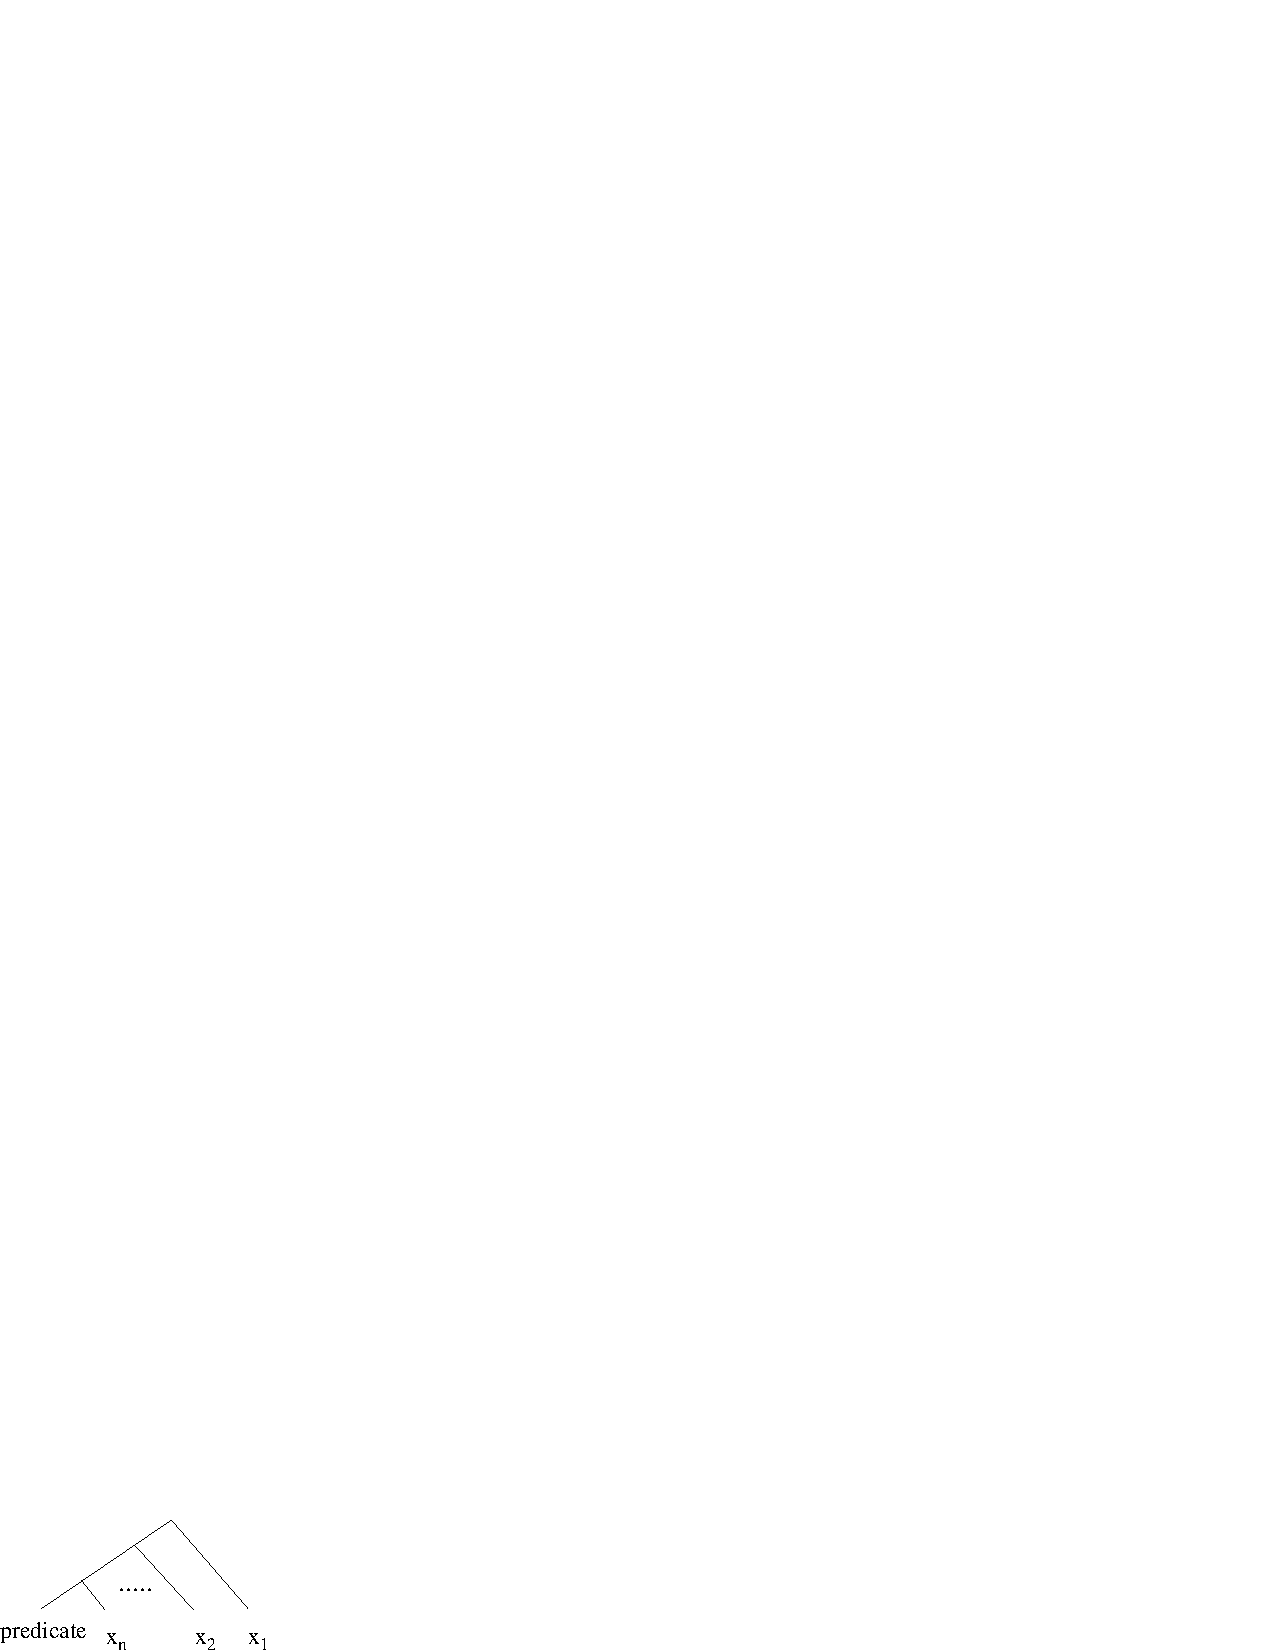
\includegraphics{pas.pdf}
\end{minipage}
\end{exe}

As we have seen earlier in this section, \occg\ uses hybrid logic
dependency semantics (HLDS) terms, rather than $\lambda$-terms, in its
logical forms. For example, the HLDS terms for (\ref{buy-lambdas}) and
(\ref{tg-catch-lambdas}) appeared in Figure~\ref{tv-lf} and in
(\ref{tg-catch}). These terms differ from their $\lambda$-counterparts
in a couple of ways. First, in semantic construction, argument binding
is accomplished through unification, rather than via function
application. And second, predicates are typically connected to their
arguments via semantic roles, such as $\modp{Agent}$ and
$\modp{Patient}$---though nothing prevents relations such as
$\modp{Arg1}$ and $\modp{Arg2}$ from being used instead. Using semantic
roles can be more convenient for applications, and makes it possible to
capture semantic similarities across argument structure alternations.
The downside is that it makes it impossible to enforce binding
constraints. In principle, relations encoding semantic roles (e.g.\
$\modp{Agent}$ and $\modp{Patient}$) could be combined with ones for
argument structure (e.g.\ $\modp{Arg1} \ldots \modp{ArgN}$) in the same
HLDS logical form, though this has not yet been tried.


\section{Types}
\label{types}

Types (aka sorts) allow for some abstraction, generalization and
specialization in an \occg\ grammar. Unlike HPSG, \occg\ only employs
atomic types. These types may be used as restrictions on syntactic or
semantic feature variables, or given as values of syntactic or semantic
features. Multiple-inheritance is allowed (see \cite{erkanms03} for
further information).

Types are kept in the types file, usually named \texttt{types.xml}. This
file is optional, which means that features can be untyped (actually,
all features will be considered to be of type \texttt{top} in this case,
which is the only predefined type). 

\begin{figure}
\begin{verbatim}
  <!-- person vals -->
  <type name="pers-vals"/>
  <type name="3rd" parents="pers-vals"/>
  <type name="non-3rd" parents="pers-vals"/>
    <type name="1st" parents="non-3rd"/>
    <type name="2nd" parents="non-3rd"/>
\end{verbatim}
\caption{Hierarchy of syntactic person values}
\label{pers-vals}
\end{figure}

In Section~\ref{words}, Figure~\ref{pers-macros}, we saw how the value
of the person feature \texttt{non-3rd} could be used to define a
category compatible with both \texttt{1st} and \texttt{2nd} person
singular subjects. This definition relies on the following specification
of person values in the \texttt{tiny} grammar's \texttt{types.xml} file,
listed in Figure~\ref{pers-vals}. As this example shows, types are
defined using a \textsl{type} element and are required to have a
\textsl{name}. They may also have a space-separated list of one or more
\textsl{parent} types. Indenting may be used to show the primary
type-subtype hierarchy:\footnote{Since multiple parents are allowed,
nesting of elements is not used to define type-subtype relationships.}
here, \texttt{1st} and \texttt{2nd} are subtypes of \texttt{non-3rd},
while \texttt{non-3rd} and \texttt{3rd} are subtypes of
\texttt{pers-vals}. If no parent types are listed---as with
\texttt{pers-vals}---the type is implicitly a subtype of \texttt{top}.

\begin{figure}
\begin{verbatim}
  <!-- ontological sorts -->
  <type name="sem-obj"/>
    <type name="phys-obj" parents="sem-obj"/>
      <type name="animate-being" parents="phys-obj"/>
        <type name="person" parents="animate-being"/>
      <type name="thing" parents="phys-obj"/>
    <type name="situation" parents="sem-obj"/>
      <type name="change" parents="situation"/>
        <type name="action" parents="change"/>
      <type name="state" parents="situation"/>
\end{verbatim}
\caption{Hierarchy of semantic types/sorts}
\label{ont-sorts}
\end{figure}

The \occg\ type system does not distinguish between syntactic and
semantic types; it is up to the grammar designer to ensure their
systematic use. For example, if there is to be a syntactic hierarchy and
a semantic hierarchy of types, it is a good idea to define a `top
object' for each (or at least for one of them), e.g.\ \texttt{sem-obj}
as the root of the semantic type hierarchy, as illustrated in
Figure~\ref{ont-sorts}. The types in this figure are the ones assumed by
the transitive verb category given in Figure~\ref{tv-lf}. With these
types, \occg\ can parse and realize \gf{he bought a flower}, but not
\gf{*a flower bought he}, since \gf{flower} has type \texttt{thing}, and
\texttt{thing} is not compatible with the type \texttt{animate-being},
as is required for the \modp{Actor} of a \C{buy} action.


\section{Rules}
\label{rules}

The rules file, typically named \texttt{rules.xml}, specifies the
combinatory rules for a grammar. The rule specifications for the
\texttt{tiny} grammar appear below:

\begin{verbatim}
  <!-- Application -->
  <application dir="forward"/>
  <application dir="backward"/>

  <!-- Harmonic Composition -->
  <composition dir="forward" harmonic="true"/>
  <composition dir="backward" harmonic="true"/>

  <!-- Crossed Composition -->
  <composition dir="forward" harmonic="false"/>
  <composition dir="backward" harmonic="false"/>

  <!-- Type-raising -->
  <typeraising dir="forward" useDollar="false"/>
  <typeraising dir="backward" useDollar="true"/>
  <typeraising dir="backward" useDollar="true">
    <arg><atomcat type="pp"/></arg>
  </typeraising>
\end{verbatim}

\noindent In addition to the rules shown here, it is also possible to
have substitution rules, as well as additional type raising rules. By
default, the argument and result categories for a type raising rule are
\cf{np} and \cf{s}, respectively. To create a type raising rule using
different categories, you can use an \textsl{arg} and/or \textsl{result}
element to specify the desired atomic category. For example, a backward
type raising rule for prepositional phrases is included as the last rule
above.

Theoretically speaking, CCG combinatory rules are universal; \emph{any}
lexicalized grammar has access to them if it uses in the lexical
categories the modalities licensed by the rules (see
\cite{Steedman/Baldridge:2003} for further information). The rules file
can also incorporate rules that are language specific. To illustrate,
let's consider the case of pro drop in Turkish. Turkish is a pro-drop
language, which means that subjects of finite clauses can be dropped
because morphology of the finite verb already indicates the subject:

\begin{itemize}
\item[(a)]
\begin{tabular}{ll}
Ben & uyu-du-m/*-n \\
I & sleep-PAST-1SG/*-2SG \\
\multicolumn{2}{l}{`I slept.'} \\
\end{tabular}

\item[(b)]
\begin{tabular}{l}
Uyu-du-m \\
sleep-PAST-1SG \\
`(I) slept.' \\
\end{tabular}
\end{itemize}

Pro drop can be modelled in different ways. For example, one can write a
lexical rule to generate the derived lexical entries of finite verbs
\emph{in} the lexicon, so that every finite verb has two lexical
entries, one derived from the other---e.g.\ (\ref{ex:prodrop}) below,
which asserts $\cf{s\fb{fin}}\bs\cf{np\fb{acc}}$ and $\cf{s\fb{fin}}$
entries in the lexicon from
$\cf{s\fb{fin}}\bs\cf{np\fb{nom}}\bs\cf{np\fb{acc}}$ and
$\cf{s\fb{fin}}\bs\cf{np\fb{nom}}$, etc.

\begin{equation}
\label{ex:prodrop}
\cf{s\fb{fin}}\bs\cf{np\fb{nom}}\$_1
\Rightarrow 
\cf{s\fb{fin}}\$_1
\end{equation}

This strategy has theoretical and practical implications. Theoretically,
it assumes that \emph{all} morphology is confined to the lexicon,
including inflectional morphology, which is usually regarded as part of
syntax (see e.g.\ \cite{bozsahin02cl} for its implications for the
transparency of syntax-semantics correspondence). \occg\ does not assume
that there are only words in the lexicon; anything that can bear a
category (words, affixes, clitics) can be a lexical
item.\footnote{Currently, \occg\ does not have any mechanism to enforce
the \emph{Lexical Integrity Principle} of \cite{bresnanmchombo95}, which
basically states that words are islands as far as syntax is concerned,
e.g.\ it is not possible to extract out of a word. \cite{bozsahin02cl}
proposes that different attachment characteristics of words and bound
morphemes can be factored into CCG's lexical entries and combinatory
rules (the latter simply projects them onto surface grammar), in effect
rendering LIP as a phonological principle, but this is an open problem
for now.}

On the practical side, it assumes that all inflected forms of the verb
are listed in the lexicon. For morphologically rich languages such as
Turkish, this amounts to around 2$^{8}$ entries per verb because Turkish
has 8 inflections in the verb paradigm, all of which are optional.

\begin{figure}
\begin{verbatim}
  <typechanging name="pd">
    <arg>
      <complexcat>
        <atomcat type="s"> 
          <fs id="1"> 
            <feat attr="v-form" val="finite"/>
          </fs>
        </atomcat>
        <slash dir="\"/>
        <atomcat type="n"> 
          <fs> <feat attr="case" val="nom"/> </fs>
        </atomcat>
      </complexcat>
    </arg>
    <result>
      <atomcat type="s"> <fs id="1"/> </atomcat>
    </result>
  </typechanging>
</rules>
\end{verbatim}
\caption{Unary rule for pro drop}
\label{pro-drop-rule}
\end{figure}

An alternative is to add a unary rule for pro drop to
\texttt{rules.xml}. This rule will apply ``on the fly'', that is, it can
apply to lexical or combinatorially-derived inflected verb forms. The
rule, which implements (\ref{ex:prodrop}), may be specified as shown in
Figure~\ref{pro-drop-rule} (we omit the \$ variable for simplicity).
Unary rules are defined using a \textsl{typechanging} element, since
such rules must change the type of the argument category---otherwise,
nothing would prevent the rule from applying again and again to its own
output.


\section{Trying it out}

Once you've configured and built \occg\, per the \texttt{README} file,
you're ready to try out the grammar testing tools. You can experiment
with the grammars described in \texttt{SAMPLE\_GRAMMARS} or make one of
your own. In the latter case, it will be easier if you create your
grammar in its own subdirectory of the \texttt{grammars} directory.

There are (at present) three command line tools for trying grammars out:
\texttt{tccg}, \texttt{ccg-test} and \texttt{ccg-realize}.

\subsection{\texttt{tccg}}

The \texttt{tccg} tool (for ``text CCG'') is for interactively testing a
grammar. Its (primary) usage is

\begin{verbatim}
  tccg (<grammarfile>)
\end{verbatim}

\noindent The default grammar file name is \texttt{grammar.xml}. You can
try it out by going to the \texttt{grammars/tiny} directory and running
\texttt{tccg}, like so:\footnote{Examples like this one may have  
an occasional extra line break to improve readability.}

\begin{small}
\begin{verbatim}
D:\Mike\dev\openccg\grammars\tiny>tccg
Loading grammar from URL: file:/D:/Mike/dev/openccg/grammars
/tiny/grammar.xml
Grammar 'tiny' loaded.

Enter strings to parse.
Type ':r' to realize selected reading of previous parse.
Type ':h' for help on display options and ':q' to quit.
You can use the tab key for command completion,
Ctrl-P (prev) and Ctrl-N (next) to access the command history,
and emacs-style control keys to edit the line.

tccg>
\end{verbatim}
\end{small}

Typing in \texttt{:h} shows all the available commands.  For example,
\texttt{:derivs} turns on the display of derivations when you parse an
expression:

\begin{small}
\begin{verbatim}
tccg> :derivs
tccg> the teacher buys
3 parses found.

Parse 1: s/np
------------------------------
(lex)  the :- np/^n
(lex)  teacher :- n
(>)    the teacher :- np
(>T)   the teacher :- s/@i(s\@inp)
(lex)  buys :- s\np/np
(>B)   the teacher buys :- s/np

tccg>
\end{verbatim}
\end{small}

\noindent Here we see a (simplified) vertical display of the derivation
seen earlier in Figure~\ref{subj-v-agr}. (If you have \LaTeX\ installed,
it's also possible to see derivations like those in
Figure~\ref{subj-v-agr} using the \texttt{:vison} command, but note that
its current behavior is a bit flaky.) Only the first parse is shown; the
other two parses, for the ditransitive and \cf{np} \cf{pp\fb{for}}
categories of the verb, can be seen by turning on all derivations with
the \texttt{:all} command. To see the features on the categories, you
can use the \texttt{:feats} command, optionally with a subset of
features to show.

Logical forms can be shown with the \texttt{:sem} command:

\begin{small}
\begin{verbatim}
tccg> :noderivs
tccg> :sem
tccg> she bought the policeman a flower
1 parse found.

Parse: s :
  @b1:action(buy ^
             <tense>past ^
             <Actor>(p1:animate-being ^ pro3f ^
                     <num>sg) ^
             <Beneficiary>(p2:person ^ policeman ^
                           <det>the ^
                           <num>sg) ^
             <Patient>(f1:thing ^ flower ^
                       <det>a ^
                       <num>sg))
tccg>
\end{verbatim}
\end{small}

To see the realizations for this logical form (i.e., the one from the 
previous parse), use the \texttt{:r} command:

\begin{small}
\begin{verbatim}
tccg> :nosem
tccg> :r
[1.000] she bought the policeman a flower :- s
[0.167] she bought a flower for the policeman :- s
tccg>
\end{verbatim}
\end{small}

\noindent Realizations are ordered by their n-gram similarity to the
previously entered expression. You can have a look in the
\texttt{morph.xml} file for more words to form expressions with.

Note that the settings of the various options available in
\texttt{tccg}; use \texttt{:reset} to undo all these settings and return
to the default ones.

\subsection{\texttt{ccg-test}}

The \texttt{ccg-test} tool is for regression testing, and also provides
options for timing the realizer. Its (primary) usage is

\begin{verbatim}
  ccg-test (-noparsing|-norealization) 
           (-g <grammarfile>) 
           (<regressionfile>)
\end{verbatim}

By default, \texttt{ccg-test} will use the grammar in the current
directory and the default regression file, \texttt{testbed.xml}.

Note that you can set realizer options, such as its time limit, in
\texttt{tccg}, e.g.\ by issuing the command \texttt{:tl 1000} (for time
limit 1000 ms.), and this value will persist and be used by
\texttt{ccg-test}.

\subsection{\texttt{ccg-realize}}

The \texttt{ccg-realize} tool provides a sample interface to the
realizer (see the underlying \texttt{opennlp/ccg/Realize.java} file),
and can be an aid in debugging realization. It loads a grammar, runs the
realizer on an input XML file, and logs its processing to an output text
file (or to system out). Its usage is

\begin{verbatim}
  ccg-realize (-g <grammarfile>) <inputfile> (<outputfile>)
\end{verbatim}
  
You can create input files for \texttt{ccg-realize} using the
\texttt{:2xml} option in \texttt{tccg}.

\section{Building grammars}

\occg\ comes with various utilities to help you build the files used by
the runtime system---and to validate their contents---rather than
writing them entirely by hand. The utilities take advantage of the
\texttt{ccg-build} front end to the Apache Ant
(\url{http://ant.apache.org}) build tool. In principle,
\texttt{ccg-build} allows you to organize your files in any way you like
to produce the runtime grammar files.

\subsection{Validating the grammar files}

You can use \texttt{ccg-build} to validate the grammar files against
their XML schemas. To do so, you need to have a \texttt{build.xml} file
in your grammar directory, which contains build tasks for the Apache Ant
tool to carry out.  The \texttt{tiny} grammar directory contains a build
file which just validates the runtime files, as shown below:

\begin{small}
\begin{verbatim}
D:\Mike\dev\openccg\grammars\tiny>ccg-build
Buildfile: build.xml

init:
     [echo] ----------- OpenCCG ------------

grammar:
     [echo] Validating grammar.xml, lexicon.xml, morph.xml, 
            rules.xml and types.xml

BUILD SUCCESSFUL
Total time: 4 seconds
\end{verbatim}
\end{small}

\noindent If there are any errors, validation with \texttt{ccg-build}
gives relatively informative error messages. Loading a grammar into
\texttt{tccg} will perform some further checks, but note that loading a
grammar with errors usually means \texttt{tccg} croaks---outputting
only (less informative) stack traces---so it's good practice to validate
any changes you make to your grammars prior to running \texttt{tccg}.

\subsection{Using a \texttt{dict.xml} file}

Rather than creating a \texttt{morph.xml} file directly, you can employ
a \texttt{dict.xml} file, which groups word forms by their stems and
parts of speech, and lists the closed families for a given stem. A
\texttt{dict.xml} files usually works together with a file called
\texttt{lexicon-base.xml}, which does not contain \textsl{member}
entries for families. From the \texttt{dict.xml} file---which also
contains macro definitions---the \texttt{morph.xml} file can be
generated automatically, with proper hooks to a derived
\texttt{lexicon.xml} file, using \texttt{ccg-build}. (See the
\texttt{dict.xsd} schema in the \texttt{grammars} directory for a
complete description.)

In short, the simplest way to use a \texttt{dict.xml} file with
\texttt{ccg-build} is to prepare a family of categories in the file
named \texttt{lexicon-base.xml} without \textsl{member} entries, and to
group stems and their word forms in a file called \texttt{dict.xml},
along with macro definitions.

A sample entry from the \texttt{cem-english} \texttt{dict.xml} 
file appears below:

\begin{verbatim}
  <entry stem="eat" pos="V">
    <member-of family="IV"/>
    <member-of family="TV"/>
    <word form="eat" macros="@nonfin"/>
    <word form="eats" macros="@pres @+3rd-agr @sg-agr"/>
    <word form="ate" macros="@past"/>
    <word form="eaten" macros="@past-part"/>
  </entry>
\end{verbatim}

\noindent Note that the stem \gf{eat} is declared intransitive and
transitive without duplication in the morph or lexicon files. If you run
\texttt{ccg-build} as follows,

\begin{verbatim}
cem-english> ccg-build grammar
Buildfile: build.xml

init:
     [echo] ----------- OpenCCG ------------

grammar:
     [echo] Adding family members from dict.xml to 
            lexicon-base.xml, yielding lexicon.xml

     [echo] Extracting morph items from dict.xml to morph.xml

     [echo] Validating grammar.xml, lexicon.xml, morph.xml, 
            rules.xml and types.xml

BUILD SUCCESSFUL
Total time: 5 seconds
\end{verbatim}

\noindent there will be two lexical assignments for every word form of
\gf{eat}, one for its intransitive use, and one for transitive.

\subsection{Reducing redundancy with XSLT}

\href{http://www.w3.org/Style/XSL/}{XSLT} is a language for transforming
XML documents. Two XSLT transformations, \texttt{add-family-members.xsl}
and \texttt{extract-morph.xsl}, are used by \texttt{ccg-build} to handle
\texttt{dict.xml} files. You can also use XSLT transformations to reduce
redundancy in the lexico-grammar specifications.

For example, the \texttt{worldcup} grammar illustrates a couple of ways
of using XSLT to improve the specification of lexical families. With
this grammar, the \texttt{lexicon-base.xml} file is generated from an
XSLT transformation, called \texttt{lexicon-base.xsl}. This file begins
with the definition of variables for the various atomic categories used
in later complex category and family definitions.  The variable names
follow the format

\begin{verbatim} 
  <cat>(.<id>)?(.from-<id>)?(.<index>?)(.<feat-descriptions>)*
\end{verbatim}

\noindent i.e., the category label, followed optionally by the
\texttt{id}, the \texttt{inheritsFrom} id, the \texttt{index} variable,
and any further feature descriptions. This convention allows one to see
what atomic categories are already in use, and to determine the contents
of an atomic category at a glance. For example, \texttt{np.3.Y.acc} is
the name of the category with label \texttt{np}, id \texttt{3}, index
\texttt{Y}, and the case value \texttt{acc}; 
\texttt{np.2.X.default} is similar, but has default variables for
all features other than the \texttt{index}.

Once variables have been declared, they can be referenced further on
using \texttt{xsl:copy-of} statements. For example, the variable
\texttt{np.2.X.default} is referenced seven times in
\texttt{lexicon-base.xsl}. In this way, if a change to
\texttt{np.2.X.default} is desired, it can be made in one place in the
file, rather than seven.

Another XSLT mechanism employed in \texttt{lexicon-base.xsl} is a named
templated called \texttt{extend} which serves to append one element as
the last child of another.  This mechanism is used to associate logical
forms with syntactic categories, as well as to create new categories
from existing ones.  For example, in

\begin{small}
\begin{verbatim} 
  <xsl:variable name="wh-det.subj">    
    <xsl:call-template name="extend">
      <xsl:with-param name="elt" 
                      select="xalan:nodeset($wh-np.subj)/*"/>
      <xsl:with-param name="ext" 
                      select="$fslash-n.2.X"/>
    </xsl:call-template>
  </xsl:variable>
\end{verbatim}
\end{small}

\noindent the category for a subject type-raised \emph{wh}-determiner,
like \gf{which}, is created by extending the category of a subject
type-raised \emph{wh}--noun phrase (e.g.\ \gf{who}) with an extra
nominal argument, \texttt{fslash-n.2.X} (declared earlier as a forward
slash plus a category with label \texttt{n}, id \texttt{2} and index
\texttt{X}).\footnote{The \texttt{xalan:nodeset} function makes it
possible to use a variable as a parameter to a named template; its use
won't be necessary in future versions of XSLT.} In this way, any changes
made to the category for \emph{wh}-determiners will carry over to the
category for \emph{wh}--noun phrases.

As XSLT is a powerful and extensible XML transformation language, there
are many further possibilities for using it in grammar
development---limited only by your imagination (and hacking ability). 

%% NB: Could eventually add lexical rule example.

%% NB: Should add discussion of chunking rules.
%% NB: Should add discussion of \textsl{licensing-features}


%% =====================================================================
%% BIBLIOGRAPHY
%% =====================================================================

\addcontentsline{toc}{section}{References}
\bibliographystyle{alpha}
\bibliography{openccg}

\end{document}

